\documentclass[serif,mathserif]{beamer}
\usepackage{etex}
\usepackage{amsmath, amsfonts, epsfig, xspace}
\usepackage{algorithm,algorithmic}
\usepackage{pstricks,pst-node}
\usepackage{multimedia}
\usepackage[normal,tight,center]{subfigure}
\usepackage{beamerthemesplit}
\usepackage{color}
\usepackage{mdframed}

\setlength{\subfigcapskip}{-.5em}
\usetheme{lankton-keynote}

\usepackage{graphicx,color}
% remove caption of figure
\usepackage[labelformat=empty]{caption}

\usepackage[none]{hyphenat} % hyphenation is ugly in slides
\usepackage{parskip}

\usepackage{relsize} % \smaller to change size

\usepackage{tikz}
\usetikzlibrary{calc}

\usetikzlibrary{arrows}

\newcommand{\TikzDraw}[2][]{
  \begin{tikzpicture}[overlay, remember picture, shift={(current page.center)}, #1]
    #2
  \end{tikzpicture}
}

\newcommand{\gridlines}{
  \TikzDraw{
    \draw[help lines,xstep=.2,ystep=.2,red!20] (current page.south west) grid (current page.north east);
    \draw[help lines,xstep=1,ystep=1,red] (current page.south west) grid (current page.north east);
    \foreach \x in {-15,-14,...,15} {
      \node [anchor=north, red] at (\x,0) {\tiny \x};
      \node [anchor=east,red] at (0,\x) {\tiny \x};
    }
  }
}

\newcommand{\DrawOnImg}[3][]
{
  \begin{tikzpicture}
    \node[anchor=south west,inner sep=0] (image) at (0,0){
      #2
    };
    \begin{scope}[x={(image.south east)},y={(image.north west)}]
      \ifthenelse{\equal{#1}{grid}}
                 {\draw[color=blue, style=dashed] (0,0) grid[xstep=.1, ystep=.1] (1.0001,1.0001);}
                 {}
                 #3
    \end{scope}
  \end{tikzpicture}
}


\author[Jiong Chen]{Jiong Chen}

\title[\hspace{2em}\insertframenumber/\inserttotalframenumber]{Large-Scale Bounded Distortion Mappings}

\date{October 28, 2015} %leave out for today's date to be insterted

% \institute{Zhejiang University}

\newcommand{\BOLD}[1]{\mathbf{#1}}
\newcommand{\BOLDG}[1]{\boldsymbol{#1}}
\newcommand{\PDIF}[2]{\frac{\partial #1}{\partial #2}}
\newcommand{\TODO}[1]{\textcolor{red}{#1}}
\newcommand{\TODOB}[1]{\textcolor{blue}{#1}}
\newcommand{\argmin}{\operatornamewithlimits{arg\min}}
\DeclareMathOperator{\tr}{tr}
\DeclareMathOperator{\cond}{cond}
\DeclareMathOperator{\ST}{s.t.}
\DeclareMathOperator{\diag}{diag}

\newmdtheoremenv{theo}{Theorem}

\definecolor{DARK}{RGB}{45, 33, 73}
\definecolor{LIGHT}{RGB}{119, 52, 106}
\definecolor{TEXTLIGHT}{RGB}{213, 207, 229}
\definecolor{TEXTDARK}{RGB}{66, 66, 66}
\definecolor{BULLET}{RGB}{179, 17, 102}
\definecolor{EM}{RGB}{179,17,102}

\begin{document}

\maketitle

\begin{frame}
 \frametitle{Problem statement}
 \begin{itemize}
  \item Given an initial map, compute a similar map whose differentials are \TODO{orientation preserving}
  and have \TODO{bounded condition number}.
  \Large
 \begin{equation*}
 \boxed{
  \begin{aligned}
    \min_{\BOLD{x}}~~&\|T\BOLD{x}-T\BOLD{x}_0\|_2  \\ 
    \ST \quad &A\BOLD{x} = \BOLD{b}\\
    &T_j\BOLD{x} \in \mathcal{D}_j
  \end{aligned}
 }
 \end{equation*}
 \large
 \item $\mathcal{D}_j=\mathcal{D}^K, j=1,2,\dots m$
 \begin{equation*}
  \det(D^K) \ge  0, \quad \cond(D^K) \le K
 \end{equation*}
 \end{itemize}
\end{frame}

\begin{frame}
 \frametitle{Problems statement}
 \begin{itemize}
  \item Non-linear and non-convex problem $\Rightarrow$ difficult \& computationally demanding
  \item Numerical methods: first-order \& second order
  \item Second order: interior point solver \& Newton variants
  \item First order 
    \begin{itemize}
     \item[-] \textcolor{red}{Alternating optimization\,(Local/global, block descent)}
     \item[-] \textcolor{green!50!black}{Gauss-Newton for least squares}
    \end{itemize}
 \end{itemize}
 \visible<2> {
  \TikzDraw {
    \draw[->, red, very thick] (-3.8, -1.2) parabola (-2, -2.4);
    \draw[->, green!50!black, very thick] (-3.8, -1.9) parabola (-2, -2.4);
    \node [fill=EM!80, draw=white, rounded corners=1mm, text opacity=1, fill opacity=10] at (-0.1, -2.8) {\Large \textcolor{white}{Efficiency \& Scalability}};
  }
 }
 %\gridlines
\end{frame}

\begin{frame}
 \frametitle{Approach}
 \TikzDraw {
  \node at (-2.7, 0) { 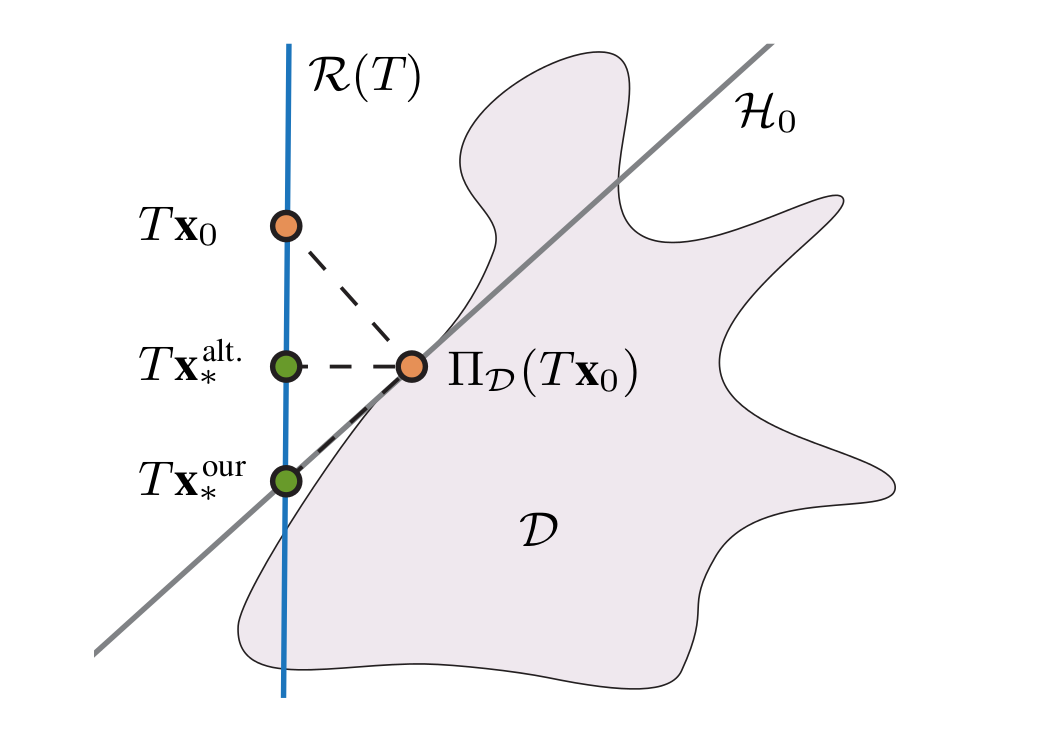
\includegraphics[scale=0.2]{img/solve} };
  \draw[fill=red] (-4.36, -1.2) circle (3pt);
  \draw[red, very thick] (-3.6, 0.18) -- (-3.8, 0) -- (-3.64, -0.18);
  \visible<2-> {
    \node at (3, 0) {\parbox[t]{0.5\textwidth}{
      Pythagorean theorem
      \begin{equation*}
      \begin{split}
	&\|T\BOLD{x}-T\BOLD{x}_0\|_2^2=\|T\BOLD{x}-\Pi_\mathcal{D}(T\BOLD{x}_0)\|^2_2 \\
	&+\|\Pi_\mathcal{D}(T\BOLD{x}_0)-T\BOLD{x}_0\|_2^2
      \end{split}
      \end{equation*}
      \begin{equation*}
       \boxed {
	\begin{aligned}
	 &\BOLD{x}_* = \argmin_\BOLD{x} \|T\BOLD{x}-\Pi_\mathcal{D}(T\BOLD{x}_0)\|_2 \\
	 &\quad\quad ~~\ST A\BOLD{x} = \BOLD{b} \\
	 &\quad\quad\quad\quad\quad T\BOLD{x} \in \mathcal{H}_0
	\end{aligned}
       }
      \end{equation*}
     }
    };
  }
 }
 \visible<3> {
  \TikzDraw {
    \draw[red, very thick] (1.8, -1.5) -- (3.8, -2.0);
    \node at (4, -2.5) {\TODO{Alternating optimization}};
  }
 }
 %\gridlines
\end{frame}

\begin{frame}
 \frametitle{Algorithmic details}
 \begin{enumerate}
  \item \textit{\textbf{Project}} the lifted variable $\BOLD{z}_n=T\BOLD{x}_n$ onto $\mathcal{D}$, \textit{i.e.}, compute $\Pi_\mathcal{D}(\BOLD{z}_n)$.
  \item Form $\mathcal{H}_n$ to be the \textbf{\textit{hyperplane}} orthogonal to the projection vector $\BOLD{z}_n-\Pi_\mathcal{D}(\BOLD{z}_n)$.
  \item \textbf{\textit{Optimize}} with $(\BOLD{x}_*, \BOLD{x}_0)=(\BOLD{x}_{n+1}, \BOLD{x}_n)$.
 \end{enumerate}
\end{frame}

\begin{frame}
 \frametitle{Projection}
 \begin{itemize}
  \item Separable projection
  \begin{equation*}
   \Pi_\mathcal{D}(\BOLD{z})=
   \begin{pmatrix}
    \Pi_{\mathcal{D}_1}(T_1\BOLD{x}) \\
    \vdots \\
    \Pi_{\mathcal{D}_m}(T_m\BOLD{x})
   \end{pmatrix}
  \end{equation*}
  \item Compute $\Pi_{\mathcal{D}_j}(T_j\BOLD{x})=\Pi_{\mathcal{D}^K}(T_j\BOLD{x})$
  \item Let $C=U\diag(\sigma_1, \dots, \sigma_d)V^T$ with $\sigma_1\ge \dots \ge \sigma_{d-1} \ge |\sigma_d|$
  \visible<1> {
  \begin{equation*}
  \boxed{
  \begin{aligned}
   &\Pi_{\mathcal{D}^K}(C) = U\diag(\tau^*_1, \dots, \tau^*_d)V^T \\
   &\{\tau^*_i\} = \argmin_{\{\tau_i\}}\sum_{i=1}^d(\sigma_i-\tau_i)^2 \\
   &\ST ~~\tau_1 \le K\tau_d
  \end{aligned}}
  \end{equation*}
  }
  \pause
  \TikzDraw {
    \visible<2> { 
      \node at (-1.2, -2.25) {$\boxed{\|\Pi_\mathcal{D}(\BOLD{z})\|_2 \le \|\BOLD{z}\|_2}$ };
      \node at (2, -2.5) {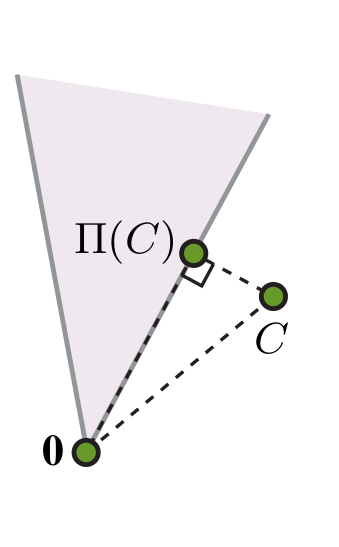
\includegraphics[scale=0.2]{img/proj}};
    }
  }
 \end{itemize}
 %\gridlines
\end{frame}

\begin{frame}
 \frametitle{Hyperplane}
 \begin{itemize}
  \item The proxy hyperplane
    \begin{itemize}
     \item[-] Passes through the projection $\Pi_\mathcal{D}(\BOLD{z}_0)$.
     \item[-] Orthogonal to the projection direction $\BOLD{n}_0=\BOLD{z}_0-\Pi_\mathcal{D}(\BOLD{z}_0)$.
    \end{itemize}
  \item 
  \begin{equation*}
    \boxed{
    T\BOLD{x}\in \mathcal{H}_0 \Rightarrow \BOLD{n}_0^T(T\BOLD{x}-\Pi_\mathcal{D}(T\BOLD{x}_0)) = 0
    }
  \end{equation*}
  \visible<1>{\item $\mathcal{H}$ provides a good linear proxy for $\mathcal{D}$ at $\Pi_\mathcal{D}(\BOLD{z})$ with tangent-like properties. \TODO{HOW GOOD?}}
  \pause
  \TikzDraw {
    \visible<2>{
      \node at (-1.2, -2.6) {\parbox{0.8\textwidth}{
	\begin{equation*}
	\boxed{
	 \begin{aligned}
	   &<\BOLD{n}_0, \BOLDG{\xi}> \le 0 \\
	   &\quad\BOLDG{\xi} = \gamma_+^{\prime}(0)
	 \end{aligned}}
	\end{equation*}
      }};
      \node at (1.5, -2.7) {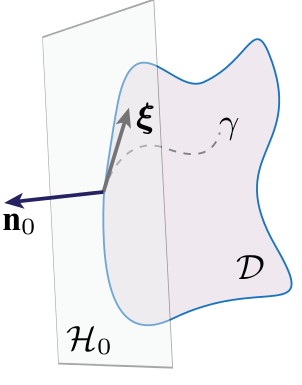
\includegraphics[scale=0.2]{img/hyper}};
    }
  }
 \end{itemize}

\end{frame}

\begin{frame}
 \frametitle{Optimize: a linear solve}
 \begin{itemize}
  \item Iteration $\Rightarrow$ solving a \textit{linearly constrained least squares problem}
  \item KKT linear system 
  \begin{equation*}
   \begin{pmatrix}
    T^TT & A^T & T^T\BOLD{n}_0 \\
    A & 0 & 0 \\
    \BOLD{n}_0^TT & 0 & 0
   \end{pmatrix}
   \begin{pmatrix}
    \BOLD{x} \\
    \BOLDG{\lambda} \\
    \mu
   \end{pmatrix}
   =
   \begin{pmatrix}
    T^TT\BOLD{x}_0 \\
    \BOLD{b} \\
    \BOLD{n}_0^T\Pi_\mathcal{D}(\BOLD{z}_0)
   \end{pmatrix}
  \end{equation*}
  \pause
  \item Schur complement
  \begin{equation*}
   \BOLDG{\eta}_0^TM^{-1}\BOLDG{\eta}_0\mu = -d_0+\BOLDG{\eta}_0^TM^{-1}\BOLD{c}_0
  \end{equation*}
  \TODOB{Only need {\LARGE{\TODO{two}}} back-substitutions}
 \end{itemize}
 \TikzDraw {
  \visible<2>{
    \draw[dashed, red, very thick](-3.2, 0.35)--(0, 0.35);
    \draw[dashed, red, very thick](0.4, 0.35)--(1.1, 0.35);
    \draw[dashed, red, very thick](1.8, 0.35)--(4.1, 0.35);
    \draw[dashed, red, very thick](-1.2, 1.3)--(-1.2, -0.2);
    \draw[orange, very thick] (-1.8, -2.27)--(-0.54, -2.27);
    \draw[orange, very thick] (1.8, -2.27)--(3.0, -2.27);
    \node at (-2.18, 0.75) {\TODO{$M$}};
    \node at (-0.6, 0.75) {\TODO{$\BOLDG{\eta}_0$}};
    \node at (-2.18, 0.1) {\TODO{$\BOLDG{\eta}^T_0$}};
    \node at (3, 0.75) {\TODO{$\BOLD{c}_0$}};
    \node at (3, 0.1) {\TODO{$d_0$}};
  }
 }
 %\gridlines
\end{frame}

\begin{frame}
 \frametitle{Remarks}
  \begin{theo}
    If $A$ is full-rank and determines global translation, and if $\BOLD{n}_0 \neq 0$ then the KKT matrix is invertible
  \end{theo}
  \begin{itemize}
    \item Proof. 
    \begin{enumerate}
     \item \TODO{$\mathcal{N}(T^TT) \cap \mathcal{N}(A) = \{0\}$} + $A$ is full-rank $\Rightarrow$ $M$ is invertible.
     \item \TODO{$\BOLD{n}_0^TT \neq 0$} $\Rightarrow$ $\BOLDG{\eta}^T_0$ is full rank + $\mathcal{N}(\BOLDG{\eta}_0^T) \cap \mathcal{N}(M) = \{0\}$
     $\Rightarrow$ KKT is invertible
    \end{enumerate}
  \end{itemize}
  \begin{itemize}
   \item Algorithm terminate $\Rightarrow$ feasible solution.
   \item Infeasible K $\Rightarrow$ no guaranteed termination.
  \end{itemize}
\end{frame}

\begin{frame}
 \frametitle{Reproduced result}
 \TikzDraw {
  \node at (0, 0) {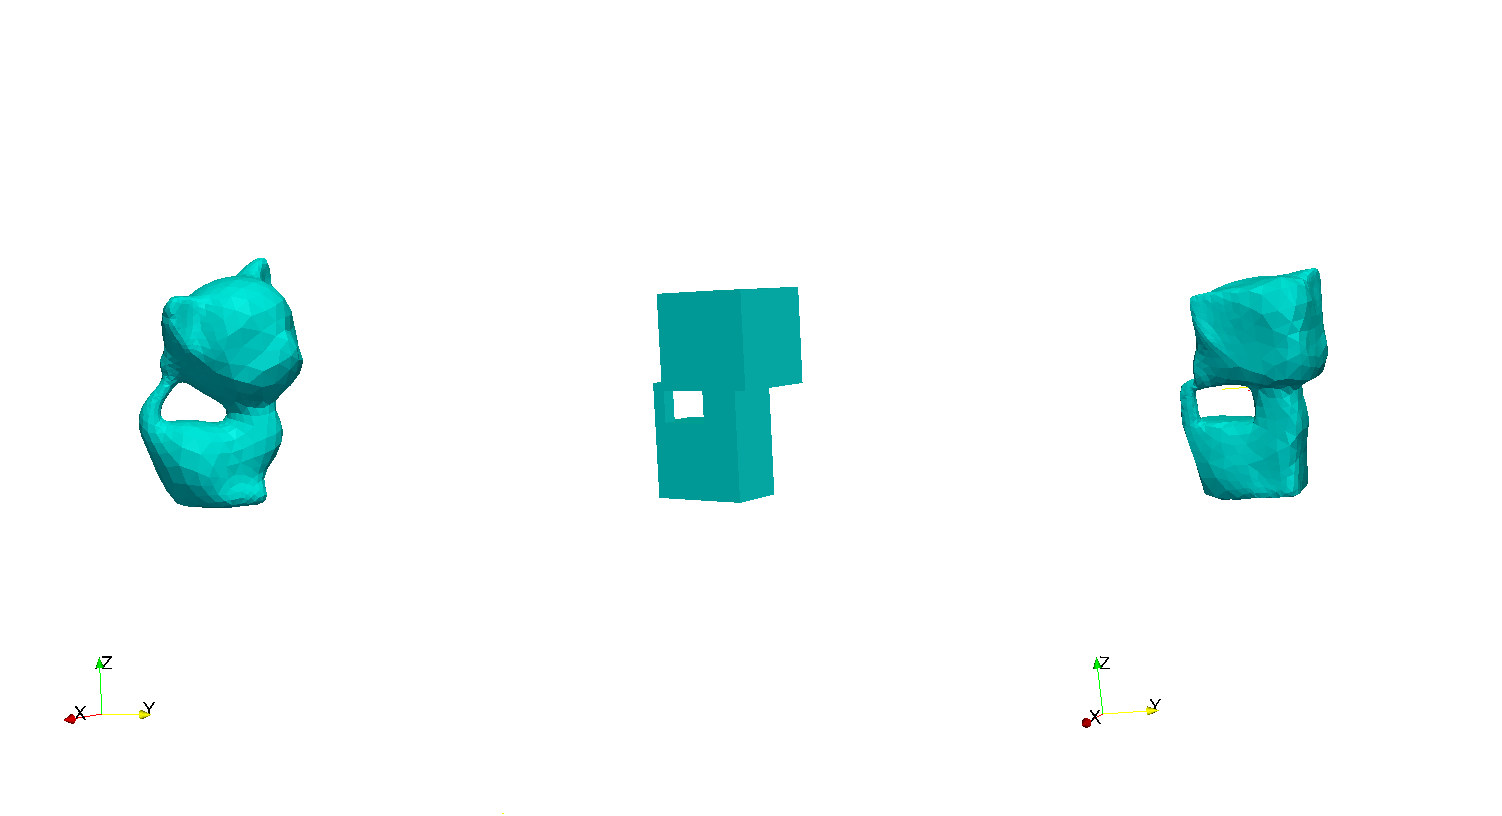
\includegraphics[scale=0.23]{img/kitty}};
  \node at (-4.2, -1.2) {source mesh};
  \node at (-0.1, -1.2) {initial mesh};
  \node at (4.1, -1.2) {$K=1.5$};
  \visible<2>{\node at (0, 0) {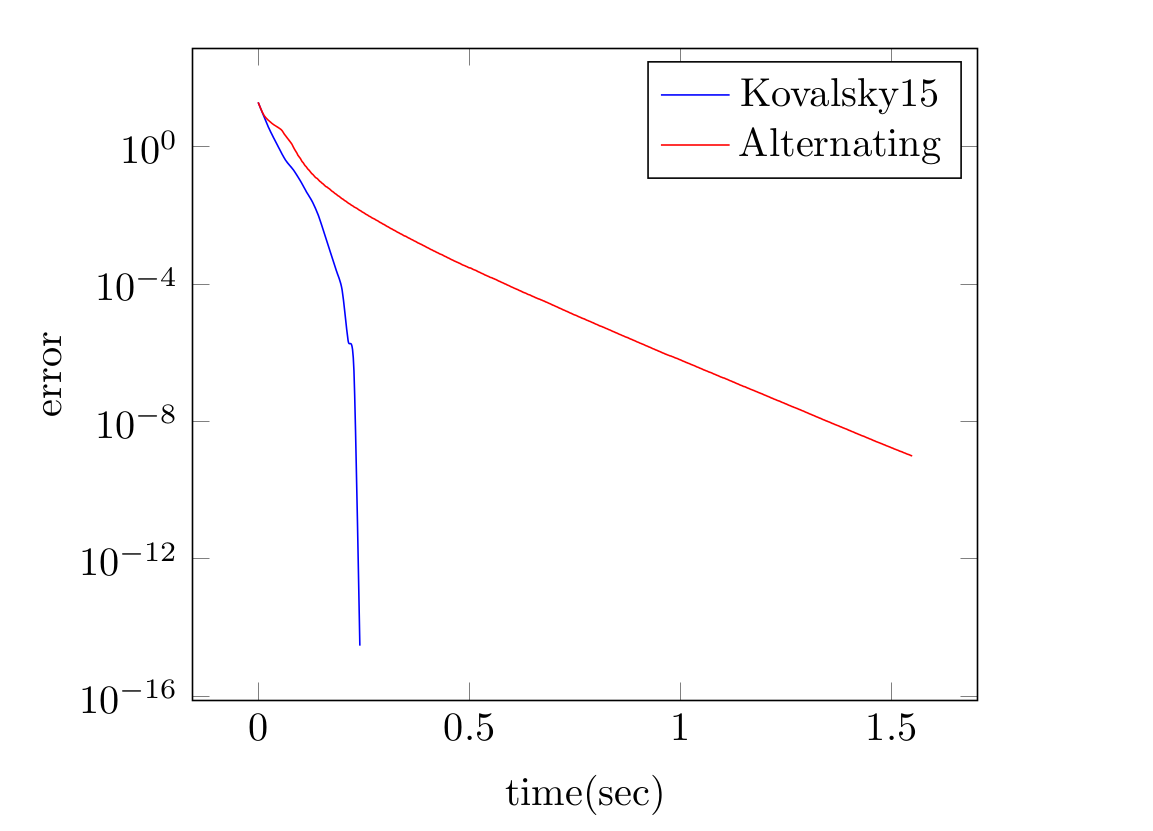
\includegraphics[scale=0.2]{img/plot}};}
 }
\end{frame}

\begin{frame}
 \frametitle{Evaluation: performance}
 \begin{figure}
  \centering
  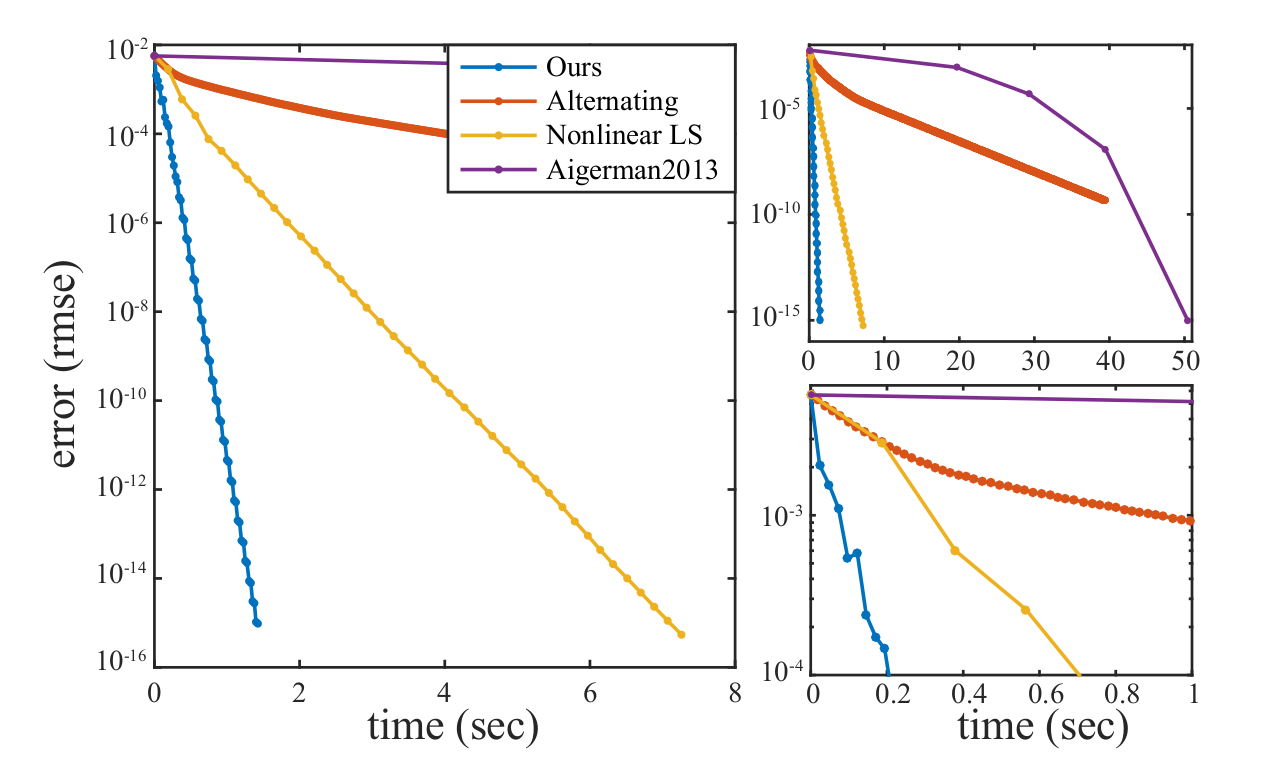
\includegraphics[width=10cm, height=5cm]{img/performance.png}
 \end{figure}
\end{frame}

\begin{frame}
 \frametitle{Evaluation: scalability}
 \begin{figure}[t]
  \centering  
  \begin{minipage}[t][0.9\textheight][s]{1\textwidth}
    \centering
    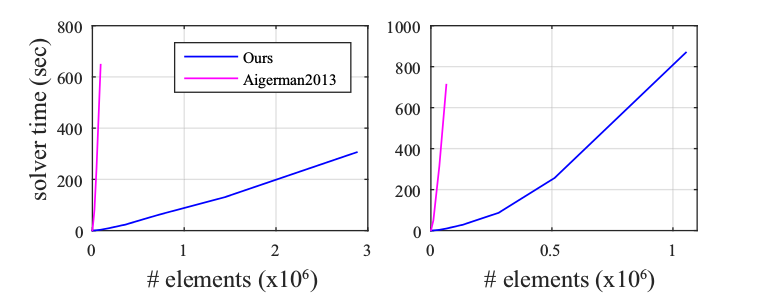
\includegraphics[scale=0.35]{img/sc0.png} 
    \vfill
    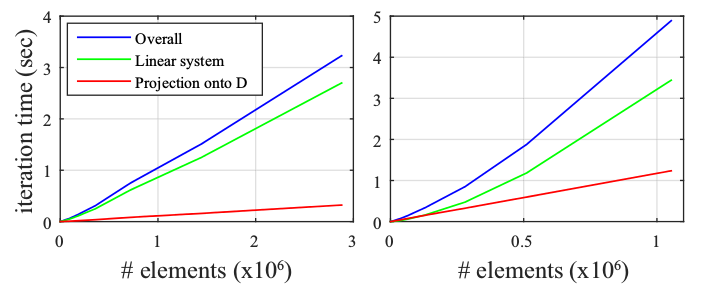
\includegraphics[scale=0.35]{img/sc1.png}
  \end{minipage}
 \end{figure}
\end{frame}

\begin{frame}
 \frametitle{Evaluation: robustness}
 \begin{figure}[t]
  \centering
  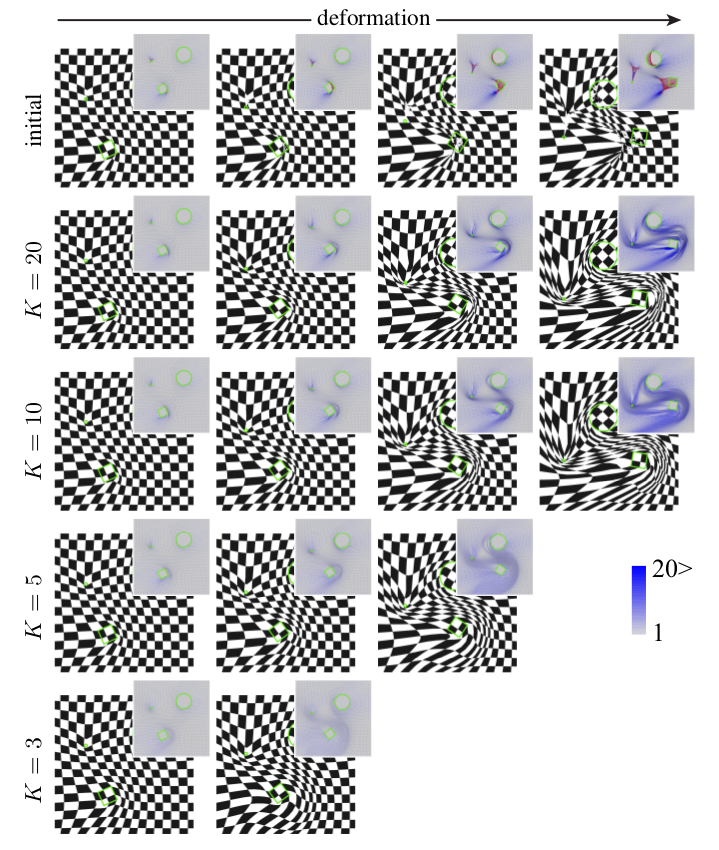
\includegraphics[width=9cm, height=8cm]{img/robustness.png}
 \end{figure}
\end{frame}

\begin{frame}
 \frametitle{More examples}
 \TikzDraw {
  \visible<2->{\node at (-2.7, -1) {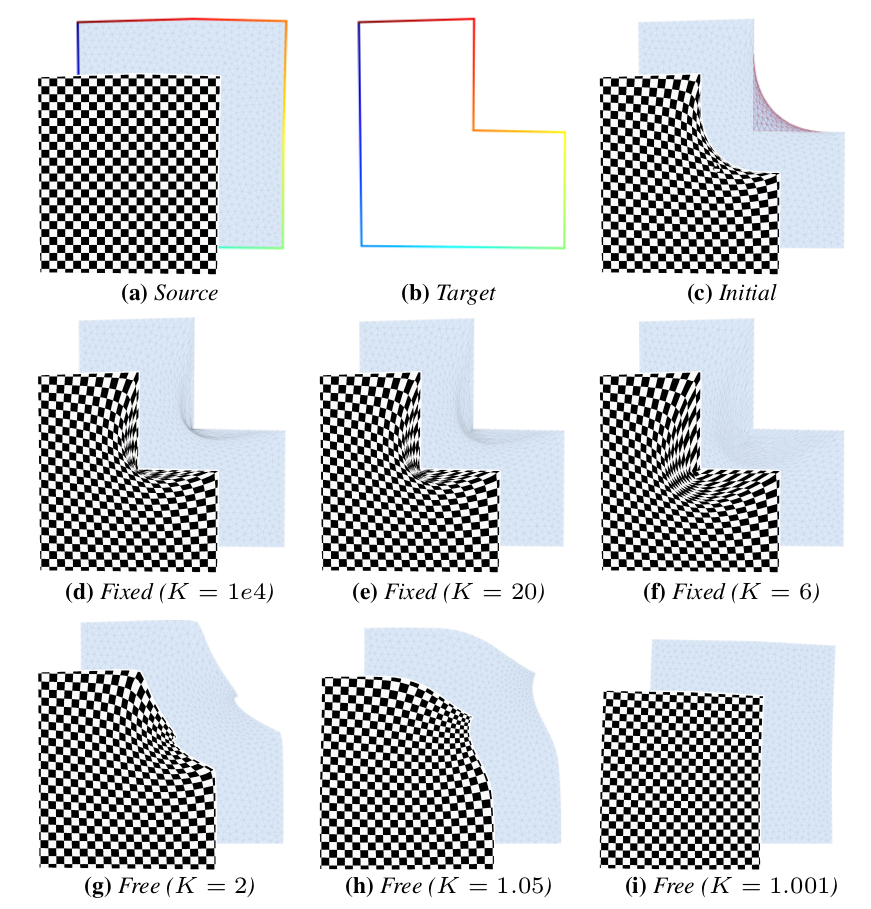
\includegraphics[scale=0.18]{img/res0}};}
  \visible<1->{\node at (-2.7, 2.8) {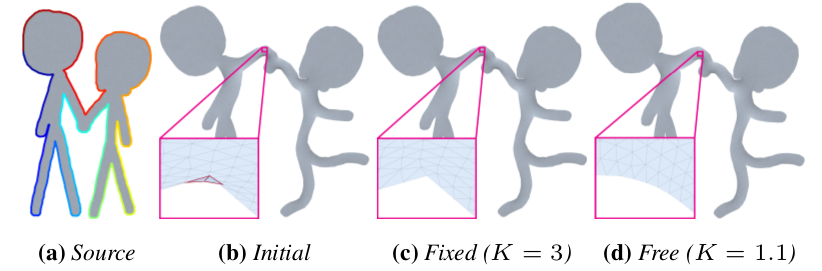
\includegraphics[scale=0.18]{img/res1}};}
  \visible<3->{\node at (3, 0.85) {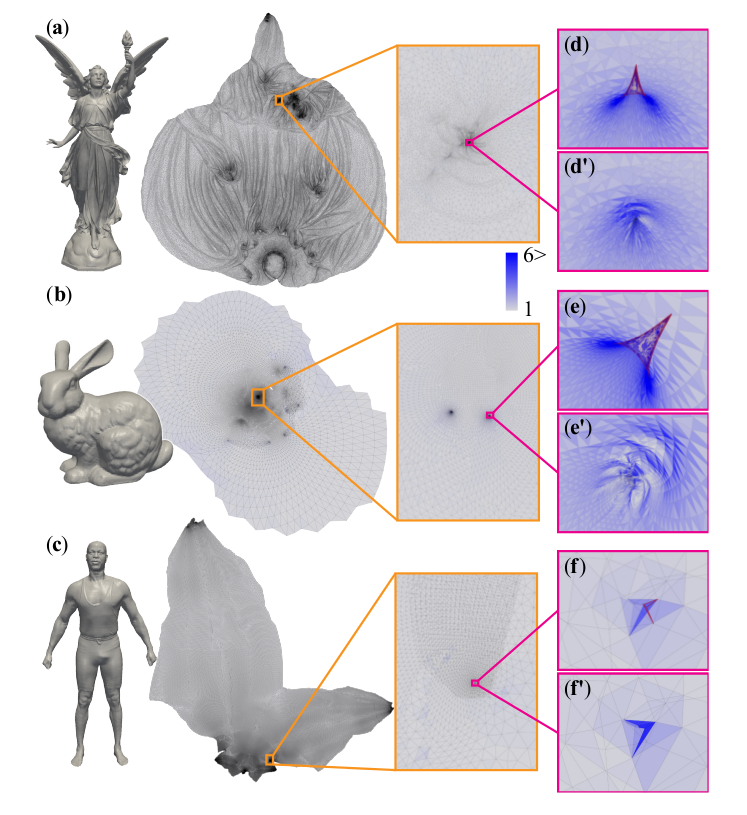
\includegraphics[scale=0.2]{img/res2}};}
  \visible<4->{\node at (3.1, -2.9) {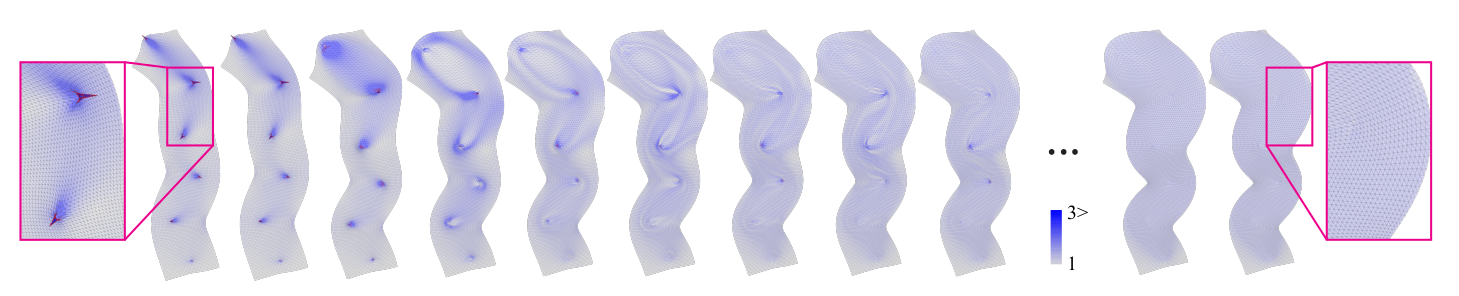
\includegraphics[width=5.2cm, height=2cm]{img/res3}};}
  \visible<5->{\node at (0, 0) {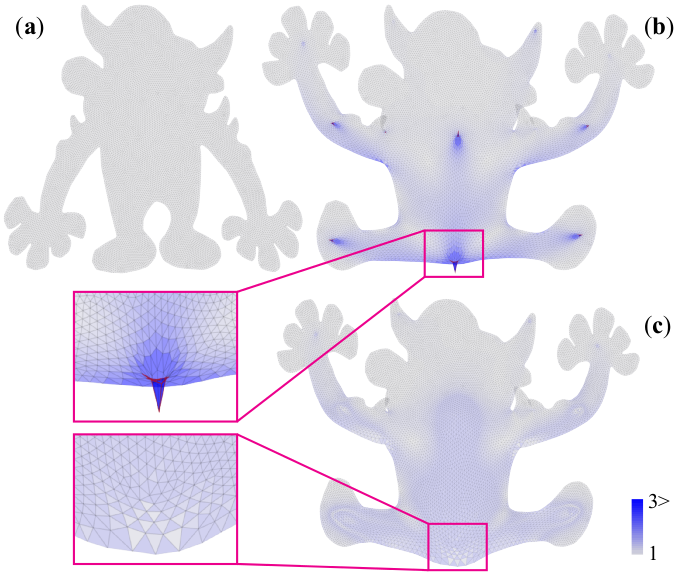
\includegraphics[scale=0.2]{img/res4}};}
 }
\end{frame}

\begin{frame}
 \frametitle{Conclusion}
 \begin{itemize}
  \item Pros:
    \begin{itemize}
      \item[-] Key: single linear hyperplane $\overset{\text{local}}{\approx}$ set of BD maps.
      \item[-] Parameter free.
      \item[-] Comparable computational efficiency to that of alternating optimization.
      \item[-] improved convergence properties. 
    \end{itemize}
  \item Cons:
    \begin{itemize}
      \item[-] Lacks global convergence guarantees.
      \item[-] Limited to mappings satisfying bounds on distortion.
  \end{itemize}
 \end{itemize}
\end{frame}

\begin{frame} 
  \TikzDraw {
    \node at (0, 0.5) {\Huge{Thanks!}};
  }
  %\gridlines
\end{frame}


\end{document}
